\chapter{Evaluation and results}

    \section{Benchmarking}
        \label{sec_benchmark}

        % the metdata benchmark is an IO benchmark. Argue this.

        Benchmarking a file system involves many aspects and different authors
        have done it in varying ways over the years.  \citeauthor{FFS} measures
        raw throughput of data, \citeauthor{LFS} recorgnise both small reads
        and writes as well as long sustained accesses.
        \citeauthor{soft_updates} on the other hands looks at speed of metadata
        access and modificaiton while \citeauthor{ext4_space_maps} uses a small
        file benchmark that simulates and email server. Finally, Google use a
        hybrid approach where they try a large variety of real world
        representative data with a large distribution of sizes. In the mean
        time popular consumer review sources add random accesses to the mix
        \cite{servethehome_review}, IO operations per second (IOPS)
        \cite{tomshardware_review} and many other ways of looking at
        performance of drives. These last methods are a bit different in that
        they measure drive performance without usually varying the filesystem
        but they are still representative as they aim to find bottlenecks and
        measure the performance of likely usecases.

        Despite the variety of test methodologies the important metrics for
        filesystems and SSDs become apparent: the raw read and write throughput
        and the number of individual IO requests they can fulfill. This is
        measured in the extremes and in various combinations of the two to
        represent different use cases like metadata access, office work or
        fileserver workloads.

        To measure these a utility written by the author of the new Linux
        system call interface io\_uring, \citeauthor{IO_uring}, is used - fio
        \cite{fio}. Using fio a test is devised to test the critical points
        that the above test for: random IO, sequential IO and metadata
        modificaiton. This is implemented as 8 'jobs' - individual tasks that
        fio completes. A Read, a write and a combined test for both small (4K
        size) and large (1M size) files, for a total of 6.  Then a sequential
        read and write test of 1GB of data and finally creating and removing
        100 files in a loop. Each of these tests is perfomerd in sequence for
        20 seconds each.

        All tests are perfomerd using the same hardware and sofware setup: a
        loopback device is set up using a regular file on the filesystem as a
        backing store. The drive is a "SAMSUNG MZVLB1T0HBLR-000L7" high speed
        NVMe drive tested on an AMD Ryzen 7 PRO 4750U CPU. The test was ran 3
        times and average values were taken. As controls two more filesystems
        were tested: ext4 and ntfs (with the ntfs-3g driver). They represent
        two of the most modern filesystems used today and are the main
        competitors to the this project (as described in section \ref{???; idk
        if i say it there}. All tests were performed by completely wiping each
        drive before commencing for consistency.

    \section{Test results}

        The results of the benchmark above are in figure \ref{fig_benchmark}.
        Combined read and write tests have the read and write components added
        toghether in the summary. The raw data for the graph can be found in
        appendinx \ref{app_benchmark}.

        % \begin{wrapfigure}{L}{0.2\textwidth}
        % \end{wrapfigure}
        \begin{figure}[h!]
            \caption{Benchmark results}
            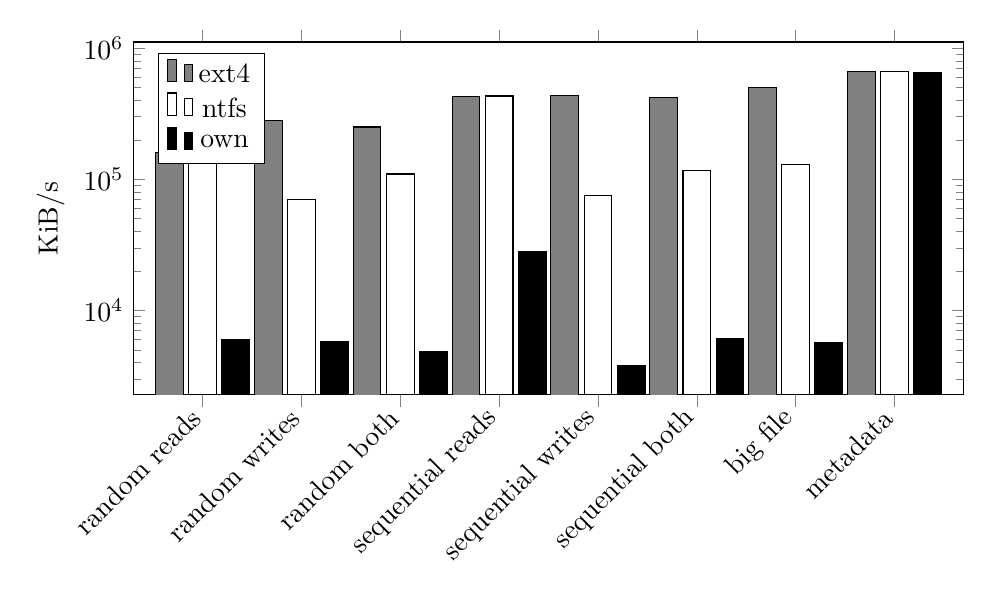
\begin{tikzpicture}
\begin{axis} [
    ybar, ymode = log,
    ylabel = {KiB/s},
    width=\textwidth, height = 0.5\textwidth,
    % scale only axis,
    symbolic x coords = {
        random reads, random writes, random both,
        sequential reads, sequential writes, sequential both,
        big file, metadata
    },
    x tick label style = {rotate = 45, anchor = east},
    legend pos = {north west}
]

    % ext
    \addplot[
        fill=gray,
    ] coordinates {
        (random reads, 159403) (random writes, 280917) (random both, 250539)
        (sequential reads, 430421) (sequential writes, 432469) (sequential both, 417792)
        (big file, 497323) (metadata, 663893)
    };

    % ntfs
    \addplot[
    ] coordinates {
        (random reads, 162133) (random writes, 70519) (random both, 109670)
        (sequential reads, 431445) (sequential writes, 74684) (sequential both, 116395)
        (big file, 128956) (metadata, 664576)
    };

    % own
    \addplot[
        fill=black,
    ] coordinates {
        (random reads, 5963) (random writes, 5812) (random both, 4820)
        (sequential reads, 28331) (sequential writes, 3799) (sequential both, 6104)
        (big file, 5693) (metadata, 651947)
    };

    \legend{ext4, ntfs, own};

\end{axis}
\end{tikzpicture}

            \label{fig_benchmark}
        \end{figure}

        The ext4 and ntfs controls appear to behave as expected. Their
        performance is comparable although ntfs performs worse across the board
        as it is natively implemented on Windows and the Linux driver has
        historically been lagging behind. Regardless, the ext4 results are a
        best case maximum whereas the ntfs ones are a more realistic
        representation of an in-kernel but imperfect filesystem.

        The proposed filesystem's performs an order of magnitude lower across
        the board. As discussed in the design stage (\ref{sec_design})
        performance was expected to be worse. Random reads and writes are of
        comparable speed. This is not surprising, as the code paths they take
        are similar. Each access needs to have its destination resolved and
        then data written in the same way. Interestingly, however, sequential
        reads are about an order of magnitude higher than the overall
        perfomance of the filesystems and the corresponding sequential writes.
        This cannot be attributed to drive assymetry, as the difference tends
        to be linear in SSDs \cite{servethehome_review}. Ext4 handles both
        workloads identially, indicating that is not the case. The ntfs-3g
        driver is a reverse engineering effort of the proprietary ntfs
        filesystem and has been notorious for having a problematic
        implementation. To confirm this, we perform profiling analysys in
        \ref{sec_perf}.

        The large file access is in line with the combined sequential test
        indicating that further increases of file size do not reduce
        performance. Finally, the metadata benchmark is surprising as it is in
        line with ext4 and ntfs. This is tahnks to directory and inode files
        having a count at the start of the file so finding a free slot is a
        very fast operation.

    \section{Profiling analysys}
        \label{sec_perf}

        To investigate why the performance is what it is the filesystem was
        profiled with perf. Perf is powerful Linux tool (part of the kernel)
        for program profiling. It can produce performance statistics for
        hardware (cache hits, idle CPU cycles etc) and for sofware (call
        graphs, call frequency, work in each subroutine etc.) \ref{perf}.

        A single profile was taken with \monospace{perf record -g
        <filesystem>}. For a workload, a full run of the benchmark was used
        \ref{sec_benchmark}. Then resulting 147Mb profile was analysed with
        \monospace{perf report -n --children} and \monospace{perf report -n
        --no-children}.

        Unsurpsiginly, most of the time is spent in the kernel (upwards of
        90\%). However, looking into which subroutine enters the kernel (with
        \monospace{--children}) has interesting results. The biggest time
        consumer is, as expected the file access subroutine
        (\monospace{do\_read\_write\_full()}).  However, in it the block
        read/write subroutines (\monospace{read\_block()} and
        \monospace{write\_block()}) do not make up even a quarter of the time
        spent. Instead, on overwhelming majority of the time is spent in btree
        accesses (\monospace{btree\_lookup64()} in this case). Upon inspecting
        the code this is due to two reasons: First, each block is located
        independently of all others and the sequential nature of the \bplustree
        is not utilised (see \ref{sec_btree} design or impl?). Second, large
        writes are handled like a sequence of small writes (with
        \monospace{do\_read\_write\_block()}). Even if sequences of blocks
        could be utilised they could not be observed by the read/write
        subroutine as it never receives them. As virtually all accesses in this
        filesystem relate to a file (\ref{sec_files}), which are accessed with
        these subroutines, all workloads behave identially porrly.

        Knowing this, to explain the sequential read anomally is not hard. With
        this arrangement reading any file will always be faster as it never
        needs to perform file expansion which requires allocation for a small
        speedup as this is un infrequent occurence. It will also, however,
        bypass the file lookup to find the inode itself to begin the read. In
        effect this removes a level of (inefficient) indirection recovering
        about half of the lost performance due to the poor use of the btrees.
        The sequential writes perform poorly because they make up the lost
        level of indirection by expanding the file in a similar manner,
        degrading performance about the same amount that was gained.

        From this analaysys there arises a corollary: allocation cannot be
        fast. And in fact this is the reason why even the largest test is
        relatively small for today's standards. Since all reads and writes are
        treated as individual requests with the size of a block, allocating a
        gigabyte of space requires about 268 million calls to the allocation
        subroutine. Since it is also slow, the results are untenable.
        % explain the 268 mil figure

        do a complexity analysys

        Benefit: simple impl. The kernel has all of that so it's fast.

% actual percents. TODO: put in listing?
% -   93.79%     0.01%            36  filesystem   filesystem            [.] do_read_write_full
%    - 93.78% do_read_write_full
%       - 93.55% do_read_write_block
%          - 86.10% get_pblock_of_byte
%             + 86.10% btree_lookup64
%          + 6.44% file_add_space
%          + 0.61% __libc_pread

        TODO: full perf availble in???
        say implementation is bad, how its bad but don't suggest anything else. That's a discussion

        IDK where to put this:

        The overall poor performance cannot be attributed to a single factor,
        but it is rather a combination of many things stacking with each other.
        First, the above mentioned sequential performance affects the entirety
        of the filesystem, including random accesses. This is beceause every
        file needs to have its inode located in the i-list. Since this is a
        single contiguous file accessing it is of sequential nature. Then, this
        file is linear. Searches through it are of linear complexity. The
        logarithmic speedup of the B-trees is irrelevant when all blocks need
        to be acccessed, especially when they are trieated as random. The same
        applies for direcoties, as their implementation is identical so
        directory lookups get a double slow down. Further, allocations slow
        things down further as described before. Finally, caching is not
        present so any neighbouring or repeat accesses are treated as
        completety independent and fresh leaving lots of performance on the
        table.

        essentially even random accesses are sequential and we already saw why those are slow

    \section{Design of the filesystem}
    % \subsection{Suitability of design as an FS}
    % maybe in discussion?

    \section{Failure simulation}

        To simulate failures we use a similar approach to the benchmarking.
        Once again, we use fio. This time a 5 minute stress test is perfomerd.
        It has two jobs which run concurrently. The first one preforms the same
        1GB combined read and write load while the second one creates and
        removes 100 files repeatedly. While this test is running a script goes
        over the first drive in the array and flips a random number of bits on
        each block up to a maximum of 100 in an infinite loop.

        As expected, the 5 minute stress test runs without any user visible
        errors. The filesystem detects and corrects all corrupt blocks and
        returns correct data stored on the redundant drives.

        % TODO: add a figure with the debug output that the error was detected and fixed

    \section{Design of the redundancy}
    % \subsection{Suitability of design for error correction}
    % \section{Reliability}

        As shown experimentally, the integrity guarantee works. Theoretically,
        best case security of the 256 bit hashes are $2^{128}$ bits.
        Theoretical attacks on reduced versions of the function put this at
        $2^{126}$ \cite{sha2_security}, \cite{sha2_analysis}. At this time
        sha-256 does not have any known collisions. So for the purposes of this
        project we consider it as secure with $2^{126}$ bits of security (we
        select the lower bound for safety).  Thus the probability that a faulty
        sector results in a hash collision will be at most $2^{-126}$. It is
        important to note that errors are not entirely arbitrary but rather
        follow some patterns \ref{the place I explain this} and are likely to
        have very few bits changed. Therefore for normal wear and tear the
        probability of a collision is likely to be much lower due to the
        avalanching effect of the funciton, however, this has not been
        theoretically verified and shall not be relied upon.

        In the event of malicious loads like a rowhammer like attack
        \cite{ssd_rowhammer} the security is likely to be lower as the attacker
        can craft the payload more carefully. However, the checksumming of the
        data provide a barrier to pulling off such an attack despite the
        lowered security (much like a canary in compilers). We can conclude
        that even if security of the hash under malicios attack is greatly
        diminished there is still a great security benefit.

        Unlike ZFS \ref{sec_ZFS}, this filesystem does not chain checksums.
        Therefore it is possible to change two blocks (one data and one hash)
        in such a way that the checksum is still valid. ZFS's chaining of
        hashes mitigates against this. However, the chance of this happening is
        astronomically low. As the errors are independent on SSDs \ref{that
        again} the likelyhood of that happening with sha256 will be $2^{252}$.
        This is a valid issue to have with short (eg. CRC) checksums however
        with long hashes this issue can be safely ignored.

        mention that the redundany will reduce even those chances

    \section{Implementation}

        As noted in the performance analysys \ref{sec_perf}, this filesystem's
        performance is not on par with what is available.  Separately, it
        experiences occasional crashes and instability, independently of the
        reliability mechanisms. As a proof of concept, this is deemed to be
        acceptable, however it should be noted that further work is required to
        develop this filesystem into a usable product.
